
\documentclass{beamer}

\usetheme{boxes}

 
\usecolortheme[RGB={34,170,34}]{structure} 
\usepackage{amsmath}
\usepackage{amssymb}
\usepackage{graphics}
\usepackage{multicol}
\usepackage{color}
\usepackage[absolute,overlay]{textpos}

\usepackage{framed,color}
\definecolor{shadecolor}{rgb}{255,127,0}
\setbeamertemplate{itemize item}[circle]

\definecolor{verde}{RGB}{34,170,34}


\setbeamercolor{uppercolgreen}{fg=white,bg=verde!90}
\setbeamercolor{lowercolgreen}{fg=black,bg=verde!20}



%%%%%%%%%%%%%%%%%%%%%%%%%%%%%%%%%%%


\title[Shell Lesson]{Loops, scripts and finding things in the shell}

\subtitle[]{EOAS Software Carpentry Workshop }
\date[Sep 2015]{September 22nd, 2015}


%------------------ the document starts here -------------------------%

\begin{document}
\bibliographystyle{plainnat}
\bibliography{bib/biblio}


%------------------ the titlepage frame-------- -------------------------%

 
\begin{frame}[plain]
  
\titlepage


\end{frame}

%-------------------------- Intro ------------------------------------------%

\begin{frame}{Loops}

\begin{figure}[htbp]
   \centering
   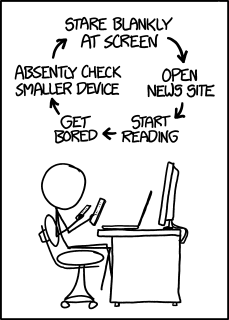
\includegraphics[width=0.45\textwidth]{figs_slides/loops.png} 
\end{figure}

\begin{textblock*}{7cm}(6.0cm,9.0cm)
		\centering
			\tiny{https://xkcd.com/1411/ }
\end{textblock*}

\end{frame}
%-------------------------- objectives ------------------------------------------%

\begin{frame}{Loops}
\begin{itemize}
    \item{Write a loop that applies one or more commands separately to each file in a set of files.}
    \item{Trace the values taken on by a loop variable during execution of the loop.}
    \item{Explain the difference between a variable�s name and its value.}
    \item{Explain why spaces and some punctuation characters shouldn�t be used in file names.}
    \item{Demonstrate how to see what commands have recently been executed.}
    \item{Re-run recently executed commands without retyping them.}
    \end{itemize}
\end{frame}


%-------------------------- Challenge 01 ------------------------------------------%

\begin{frame}{Variables in loops}
Suppose that \texttt{ls} initially displays:
\vspace{0.7cm}
\begin{beamerboxesrounded}[upper=uppercolgreen,lower=lowercolgreen,shadow=false]{}
fructose.dat      glucose.dat       sucrose.dat
\end{beamerboxesrounded}

What is the output of:
\vspace{0.7cm}
\begin{beamerboxesrounded}[upper=uppercolgreen,lower=lowercolgreen,shadow=false]{}
\texttt{for datafile in *.dat}

\texttt{do}

\texttt{	ls *.dat}

\texttt{done}
\end{beamerboxesrounded}

\end{frame}

%-------------------------- Challenge 02 ------------------------------------------%

\begin{frame}{Saving to a file in a loop }
In the same directory, what is the effect of this loop?

\begin{beamerboxesrounded}[upper=uppercolgreen,lower=lowercolgreen,shadow=false]{}
\texttt{for sugar in *.dat}

\texttt{do}

\texttt{	echo \$sugar}

\texttt{	cat \$sugar > xylose.dat}

\texttt{done}
\end{beamerboxesrounded}

\small{
\begin{enumerate}
\item{Prints \texttt{fructose.dat, glucose.dat, and sucrose.dat}, and the text from \texttt{sucrose.dat} will be saved to a file called \texttt{xylose.dat}.}
\item{Prints \texttt{fructose.dat, glucose.dat, and sucrose.dat}, and the text from all three files would be concatenated and saved to a file called \texttt{xylose.dat}.}
\item{Prints \texttt{fructose.dat, glucose.dat, sucrose.dat, and xylose.dat}, and the text from \texttt{sucrose.dat}  will be saved to a file called \texttt{xylose.dat}.}
\item{None of the above}
\end{enumerate}}


\end{frame}

%-------------------------- Challenge 03 ------------------------------------------%

\begin{frame}{Nested loops and command-line expressions}
The \texttt{expr} does simple arithmetic using command-line parameters:

\small{
\begin{beamerboxesrounded}[upper=uppercolgreen,lower=lowercolgreen,shadow=false]{}
\texttt{\$ expr 3 + 5}

\texttt{8}

\texttt{\$ expr 30 / 5 - 2}

\texttt{4}
\end{beamerboxesrounded}}

Given this, what is the output of:

\small{
\begin{beamerboxesrounded}[upper=uppercolgreen,lower=lowercolgreen,shadow=false]{}
\texttt{for left in 2   3 }

\texttt{do}

\texttt{    for right in \$left}

\texttt{     do}
 
\texttt{           expr \$left + \$right}

\texttt{     done}

\texttt{done}

\end{beamerboxesrounded}}




\end{frame}

%-------------------------- Scripts ------------------------------------------%
\begin{frame}{Scripts}
\begin{enumerate}
   \item{ Write a shell script that runs a command or series of commands for a fixed set of files.}
   \item{  Run a shell script from the command line.}
   \item{ Write a shell script that operates on a set of files defined by the user on the command line.}
   \item{  Create pipelines that include user-written shell scripts.}
\end{enumerate}
\end{frame}

%-------------------------- Challenge 01------------------------------------------%

\begin{frame}{Find the longest file with a given extension}
Write a shell script called longest.sh that takes the name of a directory and a filename extension as its parameters, and prints out the name of the file with the most lines in that directory with that extension. For example:
\vspace{0.5cm}


\begin{beamerboxesrounded}[upper=uppercolgreen,lower=lowercolgreen,shadow=false]{}
\small{\texttt{\$ bash longest.sh /tmp/data pdb}}
\end{beamerboxesrounded}

\vspace{0.5cm}

would print the name of the .pdb file in \texttt{/tmp/data} that has the most lines.
\end{frame}

%-------------------------- Challenge 02------------------------------------------%

\begin{frame}{Why record commands in the history before running them?}
If you run the command:

\vspace{0.5cm}


\begin{beamerboxesrounded}[upper=uppercolgreen,lower=lowercolgreen,shadow=false]{}
\small{\texttt{\$ history | tail -5 > recent.sh}}
\end{beamerboxesrounded}

\vspace{0.5cm}

he last command in the file is the \texttt{history} command itself, i.e., the shell has added \texttt{history} to the command log before actually running it. In fact, the shell always adds commands to the log before running them. Why do you think it does this?
\end{frame}


%-------------------------- Challenge 03------------------------------------------%

\begin{frame}{Script reading comprehension}

Joel's data directory contains three files: \texttt{fructose.dat, glucose.dat}, and \texttt{sucrose.dat}. Explain what a script called \texttt{example.sh} would do when run as bash \texttt{example.sh *.dat} if it contained the following lines:
\vspace{0.5cm}


\begin{beamerboxesrounded}[upper=uppercolgreen,lower=lowercolgreen,shadow=false]{}
\small{\texttt{\# Script 1\\
echo *.*}}
\end{beamerboxesrounded}

\begin{beamerboxesrounded}[upper=uppercolgreen,lower=lowercolgreen,shadow=false]{}
\small{\texttt{\# Script 2\\
for filename in \$1 \$2 \$3\\
do\\}
\texttt{         cat \$filename\\}
\texttt{done\\}}
\end{beamerboxesrounded}

\begin{beamerboxesrounded}[upper=uppercolgreen,lower=lowercolgreen,shadow=false]{}
\small{\texttt{\# Script 3\\
echo \$*.dat}}
\end{beamerboxesrounded}


\end{frame}

%-------------------------- Finding things ------------------------------------------%

\begin{frame}{Finding things}

\begin{enumerate}
    \item{Use grep to select lines from text files that match simple patterns.}
    \item{Use find to find files whose names match simple patterns.}
    \item{Use the output of one command as the command-line parameters to another command.}
    \item{Explain what is meant by `text' and `binary' files, and why many common tools don't handle the latter well.}
\end{enumerate}


\end{frame}

%-------------------------- Challenge 01------------------------------------------%

\begin{frame}{\texttt{find} pipeline reading comprehension}

Write a short explanatory comment for the following shell script:
\vspace{0.5cm}

\begin{beamerboxesrounded}[upper=uppercolgreen,lower=lowercolgreen,shadow=false]{}
\texttt{find . -name *.dat' -print | wc -l | sort -n}
\end{beamerboxesrounded}


\end{frame}

%-------------------------- Challenge 02------------------------------------------%

\begin{frame}{Matching \texttt{ose.dat} but not \texttt{temp}}

The \texttt{-v} flag to \texttt{grep} inverts pattern matching, so that only lines which do not match the pattern are printed. Given that, which of the following commands will find all files in \texttt{/data} whose names end in \texttt{ose.dat} (e.g., \texttt{sucrose.dat} or \texttt{maltose.dat}), but do not contain the word \texttt{temp}?


\begin{enumerate}

\item{\texttt{find /data -name `*.dat' -print | grep ose | grep -v temp}}
\item{\texttt{find /data -name \text{ose.dat} -print | grep -v temp}}
\item{\texttt{grep -v "temp" \$(find /data -name `*ose.dat' -print)}}
\item{None of the above.}

\end{enumerate}

\end{frame}

%-------------------------- the document ends here ----------------------------------%

\end{document}
